% -*- coding: utf-8 -*-
% !TEX program = xelatex

\documentclass[12pt]{beamer}

\usepackage[UTF8,noindent]{ctex}
\usepackage{arev}
\usefonttheme{professionalfonts}

\makeatletter

\providecommand{\beamer@endinputifotherversion}[1]{}

\ifxetex
  \setCJKsansfont{SimHei} % fix for ctex 2.0
  \setCJKmonofont{SimHei}
  \renewcommand\CJKfamilydefault{\CJKsfdefault}%
\else
  \@ifpackagelater{ctex}{2014/03/01}{}{\AtBeginDocument{\heiti}} %无效?
\fi

\makeatother

\renewcommand{\baselinestretch}{1} % ctex 2.4.1 开始为 1,之前为 1.3
\renewcommand{\arraystretch}{1.3}

\setlength{\parskip}{7pt plus 1pt minus 1pt}

\setbeamersize{text margin left=8mm,text margin right=8mm}

\setbeamercolor{normal text}{bg=gray!20}

\setbeamertemplate{frametitle}{\strut\insertframetitle\strut\par}
\setbeamertemplate{navigation symbols}{}

\newcommand{\cdotfill}{\leavevmode\xleaders\hbox to 0.5em{\hss$\cdot$\hss}\hfill\kern0pt\relax}

\usepackage{tabularx}

\newcommand{\ulinefill}[1]{\xleaders\hbox{\underline{\vphantom{#1}\kern1pt}}\hfill\kern0pt}
\newcommand{\fillbox}[1]{\ulinefill{#1}\underline{#1}\ulinefill{#1}}

\setbeamertemplate{title page}{%
  \renewcommand{\arraystretch}{2}%
  \usebeamerfont{title}
  \begin{tabularx}{\linewidth}{|X|}
    \hline
    模板名称:\fillbox{\usebeamercolor[fg]{title}\inserttitle} \\
    模板作者:\fillbox{\insertauthor} \\
    所在单位:\fillbox{\insertinstitute} \\
    更新日期:\fillbox{\the\year}年\fillbox{\the\month}月\fillbox{\the\day}日\\
    \hline
  \end{tabularx}%
}

\usepackage{ragged2e}

\justifying
\let\oldraggedright\raggedright
\let\raggedright\justifying

\usepackage{fancyvrb}

\newenvironment{framex}{\begin{frame}[fragile=singleslide,environment=framex]}{\end{frame}}

\DefineVerbatimEnvironment{code}{Verbatim}{%
  formatcom=\color{blue!50!red}%
}

\begin{document}

\title{暨南大学试卷 LaTeX 模板}
\author{吕\ 荐\ 瑞}
\institute{暨南大学数学系}

\begin{frame}[plain]
\titlepage
\end{frame}

\section{模板介绍}

\begin{framex}
\frametitle{简单介绍}
本文档介绍 \verb!jnuexam! 文档类。这个文档类提供暨南大学考试试卷的 LaTeX 模板。
\par
这个模板将格式和内容分开,而且可以从一份 \verb!tex! 文件编译出四份试卷(A卷 / B卷 / A卷答案 / B卷答案),使用方便。
\par
这个模板的最新版本可以在下面地址下载:\newline
 \color{blue}{\href{https://lvjr.bitbucket.io/jnuexam.html?\the\year}{\ttfamily https://lvjr.bitbucket.io/jnuexam.html}}
\end{framex}

\begin{framex}
\frametitle{编译方式}
这个文档类要求所有 \verb!tex! 文件都使用 \verb!UTF8! 编码,
若使用 \verb!GBK! 编码则无法得到正确结果。
\par
如果对文件编码不熟悉,可以直接复制例子文件,然后在其中修改,即可正常编译。
\par
这个文档类同时支持 \verb!XeLaTeX! 和 \verb!PDFLaTeX! 方式编译。为得到最好的中文显示效果,
推荐用较先进的 \verb!XeLaTeX! 编译。
\end{framex}

\section{试卷结构}

\begin{framex}
\frametitle{试卷结构}
下面是 \verb!jnuexam! 试卷文档的基本结构:
\begin{code}
\documentclass{jnuexam}
% 导言区
\begin{document}
% 正文区
\end{document}
\end{code}
导言区用于设定装订线和草稿纸等等选项。\par
正文区用于填写试卷表头和输入试卷内容。
\end{framex}

\begin{framex}
\frametitle{装订草稿}
在文档的导言区可以设定装订线和草稿纸。比如:
\begin{code}
\setexam{
  binding = 2, % 装订线
  scratch = 1, % 草稿纸
}
\end{code}
其中 \verb!binding! 取 0 表示没有装订线,
取 1 表示仅空白试卷有,取 2 表示空白试卷和试卷答案都有。\par
而 \verb!scratch! 的取值表示草稿纸数量,以 A3 大小双面印刷计算。
草稿纸仅在空白试卷中出现,试卷答案里不会带草稿纸。
\end{framex}

\begin{framex}
\frametitle{试卷正文}
\begin{code}
\documentclass{jnuexam}
\begin{document}
......
\makehead %生成试卷表头
......
\makepart{填空题}{题数分值}
......
\makepart{单选题}{题数分值}
......
\makepart{计算题}{题数分值}
......
\makepart{证明题}{题数分值}
......
\makedata{可能用到的数据} %附录数据
......
\end{document}
\end{code}
\end{framex}

\begin{framex}
\frametitle{试卷表头}
\begin{code}
\renewcommand{\niandu}{2010--2011}
\renewcommand{\xueqi}{2}
\renewcommand{\kecheng}{大学数学}
\renewcommand{\zhuanye}{理工4学分}
\renewcommand{\jiaoshi}{某某某}
\renewcommand{\shijian}{2011年07月08日}
\renewcommand{\bixiu}{1}   % 1为必修,0为选修
\renewcommand{\bijuan}{1}  % 1为闭卷,0为开卷
\renewcommand{\shijuan}{A} % A/B/C卷
\renewcommand{\neizhao}{1} % 1打勾,0不勾
\renewcommand{\waizhao}{0} % 1打勾,0不勾
\makehead %生成试卷表头
\end{code}
其中 \verb!\zhuanye! 和 \verb!\shijian! 命令的内容可以为空。
\end{framex}

\begin{framex}
\frametitle{判断题目}
\begin{code}
\makepart{判断题}{题数分值}

\begin{problem}
第一道判断题描述。\tickout{t}
\end{problem}

\begin{problem}
第二道判断题描述。\tickout{f}
\end{problem}
\end{code}
其中 \verb!\tickout{t}! 和 \verb!\tickout{f}!
分别表示打勾(\textcolor{blue}{$\checkmark$})和打叉(\textcolor{blue}{\large$\times$})。
还可用大写的 \verb!\tickout{T}! 和 \verb!\tickout{F}!,
分别表示输出 \textcolor{blue}{\textsf{T}} 和 \textcolor{blue}{\textsf{F}}。
\par
答案必须放在 \verb!\tickout! 命令里;这样才能在生成空白试卷时隐藏它。
\end{framex}

\begin{framex}
\frametitle{填空题目}
\begin{code}
\makepart{填空题}{题数分值}

\begin{problem}
第一道填空题描述\fillout{答案}。
\end{problem}

\begin{problem}
第二道填空题描述\fillout{答案}。
\end{problem}
\end{code}
\verb!\fillout! 命令将用下划线填满整行。另有个 \verb!\fillin! 命令,只留下最小宽度的下划线。
\par
答案必须放在 \verb!\fillout! 或 \verb!\fillin! 命令里面;这样才能在生成空白试卷时隐藏它。
\end{framex}

\begin{framex}
\frametitle{选择题目}
\begin{code}
\makepart{单选题}{题数分值}

\begin{problem}
第一道单选题描述\pickout{答案}。
\end{problem}

\begin{problem}
第二道单选题描述\pickout{答案}。
\end{problem}
\end{code}
\verb!\pickout! 命令将把选择圆括号放在本行最右边。另外有个 \verb!\pickin! 命令,将选择圆括号放在当前位置。
\par
答案必须放在 \verb!\pickout! 或 \verb!\pickin! 命令里面;这样才能在生成空白试卷时隐藏它。
\end{framex}

\begin{framex}
\frametitle{选项排版}
选择题的四个选项可以用 \verb!abcd! 环境来排版。比如:
\begin{code}
\begin{abcd}
  \item 第一个选项
  \item 第二个选项
  \item 第三个选项
  \item 第四个选项
\end{abcd}
\end{code}
此时 \verb!abcd! 环境将根据各选项长度自动将四个选项分为一行、两行或四行排版,非常方便。
\end{framex}


\begin{framex}
\frametitle{答题表格}
在填空题和选择题前面,还可以用 \verb!\answertable! 命令生成空白答题栏。比如:
\begin{code}
\answertable[3em]{6}{3}
\end{code}
其中 \verb!\answertable! 命令的三个参数含义如下:
\begin{itemize}
  \item 第一个可选参数表示空白单元格的高度,默认是 \verb!1em!。
  \item 第二个必选参数表示总共有多少个题目。
  \item 第三个必选参数表示每行排版几个题目。
\end{itemize}
\end{framex}

\begin{framex}
\frametitle{计算题目}
\begin{code}
\makepart{计算题}{题数分值}

\begin{problem}
第一道计算题描述。
\end{problem}
\begin{solution}
第一道计算题答案。
\end{solution}

\begin{problem}
第二道计算题描述。
\end{problem}
\begin{solution}
第二道计算题答案。
\end{solution}
\end{code}
\end{framex}

\begin{framex}
\frametitle{证明题目}
\begin{code}
\makepart{证明题}{题数分值}

\begin{problem}
第一道证明题描述。
\end{problem}
\begin{solution}
第一道证明题答案。
\end{solution}

\begin{problem}
第二道证明题描述。
\end{problem}
\begin{solution}
第二道证明题答案。
\end{solution}
\end{code}
\end{framex}

\begin{framex}
\frametitle{解答名称}
通过重新定义 \verb!\solutionname! 命令,可以改变 \verb!solution! 环境的名称。
比如下面例子将“解答”二字改为“证明”:
\begin{code}
\renewcommand{\solutionname}{证明}
\end{code}
\end{framex}

\begin{framex}
\frametitle{评分命令}
计算题和证明题等主观题的排版方法是完全一样的。在编写这些主观题的解答时,
可以用 \verb!\points! 命令给出各步骤得分。比如:
\begin{code}
\begin{solution}
$1+1=2$ \points{4}
$2+2=4$ \points{8}
\end{solution}
\end{code}
评分命令 \verb!\points! 也可在 \verb!align*! 等数学环境中使用,此时评分显示在公式编号位置。
\end{framex}

\begin{framex}
\frametitle{对齐命令}
此文档类提供几个对齐命令,用于在不同行之间对齐。比如
\vskip1em\hrule
我们有$(a+b)^2 = (a+b)(a+b)$ \par
\leavevmode\phantom{我们有$(a+b)^2$}${}= a^2 + 2ab + b^2$ \hfill$\cdots\cdots$ 2分
\vskip0.6em\hrule\vskip1em
\begin{code}
我们有$(a+b)^2 \? = (a+b)(a+b)$ \\
               \+$= a^2+2ab+b^2$ \points{2}
\end{code}
第一个公式内部的 \verb!\?! 保存当前水平位置,
而第二个公式前面的 \verb!\+! 表示跳到之前保存的位置。
\par
这两个对齐命令 \verb!\?! 和 \verb!\+! 需要编译两次才能生效。
\end{framex}

\begin{framex}
\frametitle{对齐命令}
此文档类提供几个对齐命令,用于在不同行的对齐。比如
\vskip1em\hrule
我们有$(a+b)^2 = (a+b)(a+b)$ \par
\leavevmode\phantom{我们\,}${}= a^2 + 2ab + b^2$ \hfill$\cdots\cdots$ 2分
\vskip0.6em\hrule\vskip1em
\begin{code}
我们有 \? $(a+b)^2 = (a+b)(a+b)$ \\
      \< $= a^2+2ab+b^2$ \points{2}
\end{code}
第一行公式前面的 \verb!\?! 保存当前水平位置,
而第二行公式前面的 \verb!\<! 表示跳到之前保存位置的左侧(左移一个等号的宽度)。
\par
这两个对齐命令 \verb!\?! 和 \verb!\<! 需要编译两次才能生效。
\end{framex}

\begin{framex}
\frametitle{其它题型}
除了上述四种题型之外,其它题型可以用下面方式编写:
\begin{code}
\makepart{某题型}{题数分值}

\begin{problem}
第一题描述。\answer{第一题答案}
\end{problem}

\begin{problem}
第二题描述。\answer{第二题答案}
\end{problem}
\end{code}
其中题目答案必须放在 \verb!\answer! 命令里面;这样才能在生成空白试卷时隐藏它。
\end{framex}

\begin{framex}
\frametitle{附录数据}
在试卷最后,可以用下面命令增加附录数据部分:
\begin{code}
\makedata{可能用到的数据} %附录数据
......
\end{code}
附录数据必须放在 \verb!\makedata! 命令后面;否则在从A卷生成B卷时会出问题。
\end{framex}

\section{模板选项}

\begin{framex}
\frametitle{空白试卷}
假设 \verb!exam-a-answer.tex! 是含答案的试卷。新建一个包含以下内容的 \verb!exam-a-empty.tex! 文档,
编译后将得到不含答案的空白试卷。
\begin{code}
\PassOptionsToClass{noanswer}{jnuexam}
% -*- coding: utf-8 -*-
% !TEX program = xelatex
\documentclass{jnuexam}

%\answerfalse %不显示答案

\setexam{
  binding = 2, % 装订线,1 仅空白试卷有,2 试卷和答案都有
  scratch = 1, % 草稿纸数量,仅空白试卷有,A3 大小,双面印刷
}

\begin{document}

\renewcommand{\niandu}{2017--2018}
\renewcommand{\xueqi}{2}
\renewcommand{\kecheng}{大学数学}
\renewcommand{\zhuanye}{理工四学分} % 可以为空白
\renewcommand{\jiaoshi}{张三,李四,王五} % 教师姓名
\renewcommand{\shijian}{2018~年~06~月~28~日}
\renewcommand{\bixiu}{1} % 1 为必修,0 为选修
\renewcommand{\bijuan}{1} % 1 为闭卷,0 为开卷
\renewcommand{\shijuan}{A} % A 或 B 或 C 卷
\renewcommand{\neizhao}{1} % 1 打勾,0 不勾
\renewcommand{\waizhao}{0} % 1 打勾,0 不勾

\makehead % 生成试卷表头

\makepart{填空题}{共~6~小题,每小题~3~分,共~18~分}

\answertable[3em]{6}{3} % 生成答题栏:行高3em,总共6题,每行3题

\newpageb % B卷分页点

\begin{problem}
设常数$k>0$,函数$f(x)=\ln x-\dfrac{x}{\e}+k$在$(0,+\infty)$内零点的个数为 \fillout{$2$}.
\end{problem}

\vfill

\begin{problem}
设$\va=(2,1,2)$,$\vb=(4,-1,10)$,$\vc=\vb-\lambda\va$,且$\va\bot\vc$,则$\lambda=$ \fillout{$3$}.
\end{problem}

\vfill

\begin{problem}
已知二阶行列式 $\left|\begin{array}{cc}
  1 & 2\\
  - 3 & x
\end{array}\right|=0$,则 $x=$ \fillout{$-6$}.
\end{problem}

\vfill

\begin{problem}
向量组 $\alpha_1=(1,1,0), \alpha_2=(0,1,1), \alpha_3=(1,0,1)$,
则将向量 $\beta=(4, 5, 3)$ 表示为 $\alpha_1, \alpha_2, \alpha_3$
的线性组合为 $\beta=$ \fillout{$3\alpha_1+2\alpha_2+\alpha_3$}.
\end{problem}

\vfill

\begin{problem}
已知随机变量$\xi$的期望和方差各为$E\xi=3, D\xi=2$, 则$E\xi^2=$ \fillout{$11$}.
\end{problem}

\vfill

\begin{problem}
已知$\xi$和$\eta$相互独立且$\xi\sim N(1,4), \eta\sim N(2,5)$,则$\xi-2\eta\sim$ \fillout{$N(-3,24)$}.
\end{problem}

\vfill

\newpagea % A卷分页点

\makepart{单选题}{共~6~小题,每小题~3~分,共~18~分}

\answertable{6}{6} % 生成答题栏:默认行高,总共8题,每行8题

\newpageb % B卷分页点

\begin{problem}
在下列等式中,正确的结果是\pickout{C}
\begin{abcd}
\item $\int f'(x)\dx=f(x)$
\item $\int \d f(x)=f(x)$
\item $\frac{\d}{\dx}\big(\int f(x)\dx\big)=f(x)$
\item $\d\big(\int f(x)\dx\big)=f(x)$
\end{abcd}
\end{problem}

\bigskip

\begin{problem}
假设$F(x)$是连续函数$f(x)$的一个原函数,则必有\pickout{A}
\begin{abcd}
\item $F(x)$是偶函数 $\Leftrightarrow$ $f(x)$是奇函数
\item $F(x)$是奇函数 $\Leftrightarrow$ $f(x)$是偶函数
\item $F(x)$是周期函数 $\Leftrightarrow$ $f(x)$是周期函数
\item $F(x)$是单调函数 $\Leftrightarrow$ $f(x)$是单调函数
\end{abcd}
\end{problem}

\bigskip

\begin{problem}
设矩阵 $A = \left(\begin{array}{ccc}
  1 & 1 & 0\\
  1 & x & 0\\
  0 & 0 & 1
\end{array}\right)$ 其中两个特征值为 $\lambda_1 = 1$ 和 $\lambda_2
= 2$,则 $x=$ \pickout{B}
\begin{abcd}
\item $2$
\item $1$
\item $0$
\item $-1$
\end{abcd}
\end{problem}

\bigskip

\begin{problem}
二次型 $f = 4 x_1^2 - 2 x_1 x_2 + 6 x_2^2$ 对应的矩阵等于 \pickout{C}
\begin{abcd}
\item $\left(\begin{array}{cc}
  4 & - 2\\
  - 2 & 6
\end{array}\right)$
\item $\left(\begin{array}{cc}
  2 & - 2\\
  - 2 & 3
\end{array}\right)$
\item $\left(\begin{array}{cc}
  4 & - 1\\
  - 1 & 6
\end{array}\right)$
\item $\left(\begin{array}{cc}
  2 & - 1\\
  - 1 & 3
\end{array}\right)$
\end{abcd}
\end{problem}

\bigskip

\begin{problem}
下列说法\CJKunderline{不正确}的是\pickout{B}
\begin{abcd}
\item 大数定律说明了大量相互独立且同分布的随机变量的均值的稳定性
\item 大数定律说明大量相互独立且同分布的随机变量的均值近似于正态分布
\item 中心极限定理说明了大量相互独立且同分布的随机变量的和的稳定性
\item 中心极限定理说明大量相互独立且同分布的随机变量的和近似于正态分布
\end{abcd}
\end{problem}

\bigskip

\begin{problem}
对总体$X$和样本$(X_1,\cdots,X_n)$的说法哪个是\CJKunderline{不正确}的\pickout{D}
\begin{abcd}
\item 总体是随机变量
\item 样本是$n$元随机变量
\item $X_1, \cdots, X_n$相互独立
\item $X_1 = X_2 =\cdots = X_n$
\end{abcd}
\end{problem}

\bigskip

\newpagea % A卷分页点

\makepart{计算题}{共~6~小题,每小题~8~分,共~48~分}

\newpageb % B卷分页点

\begin{problem}
求不定积分$\displaystyle\int\e^{2x}\,(\tan x+1)^2\dx$。
\end{problem}

\smallskip

\begin{solution}
\everymath{\displaystyle}%
原式 \? $=\int\e^{2x}\,\sec^2 x\dx+2\int\e^{2x}\,\tan x\dx$ \points{2}
\+ $=\int\e^{2x}\,\d(\tan x)+ 2\int\e^{2x}\,\tan x\dx$ \points{4}
\+ $=\e^{2x}\,\tan x - 2\int\e^{2x}\,\tan x\dx+ 2\int\e^{2x}\,\tan x\dx$ \points{6}
\+ $=\e^{2x}\,\tan x + C$ \points{8}
\end{solution}

\vfill

\begin{problem}
求过点$A(1,2,-1), B(2,3,0),C(3,3,2)$ 的三角形$\triangle ABC$ 的面积和它们确定的平面方程.
\end{problem}

\smallskip

\begin{solution}
由题设$\overrightarrow{AB}=(1,1,1),\overrightarrow{AC}=(2,1,3)$, \points{2}
故$\overrightarrow{AB}\times \overrightarrow{AC}=\begin{vmatrix}
\vec{i}&\vec{j} &\vec{k}\\
1&1&1\\
2&1&3\\
\end{vmatrix}=(2,-1,-1)$, \points{4}
三角形$\triangle ABC$ 的面积为$S_{\triangle ABC}=\dfrac{1}{2}\big|\overrightarrow{AB}\times
\overrightarrow{AC}\big|=\dfrac{1}{2}\sqrt{6}.$ \points{6}
所求平面的方程为$2(x-2)-(y-3)-z=0$, 即$2x-y-z-1=0$ \points{8}
\end{solution}

\vfill

\newpage % A,B卷共同分页点

\begin{problem}
计算四阶行列式 $A = \left|\begin{array}{cccc}
  0 & 1 & 2 & 3\\
  1 & 2 & 3 & 0\\
  2 & 3 & 0 & 1\\
  3 & 0 & 1 & 2
\end{array}\right|$ 的值.
\end{problem}

\smallskip

\begin{solution}
$A \? = \left|\begin{array}{cccc}
    0 & 1 & 2 & 3\\
    1 & 2 & 3 & 0\\
    2 & 3 & 0 & 1\\
    3 & 0 & 1 & 2
  \end{array}\right| = \left|\begin{array}{cccc}
    0 & 1 & 2 & 3\\
    1 & 2 & 3 & 0\\
    0 & - 1 & - 6 & 1\\
    0 & - 6 & - 8 & 2
  \end{array}\right| = 1 \cdot (- 1)^{2 + 1} \left|\begin{array}{ccc}
    1 & 2 & 3\\
    - 1 & - 6 & 1\\
    - 6 & - 8 & 2
  \end{array}\right|$ \points{4}
\+ $= -\left|\begin{array}{ccc}
    1 & 2 & 3\\
    0 & - 4 & 4\\
    0 & 4 & 20
  \end{array}\right| = - \left|\begin{array}{cc}
    - 4 & 4\\
    4 & 20
  \end{array}\right| = -(-4\cdot20-4\cdot4) = 96$ \points{8}
\end{solution}

\vfill

\begin{problem}
利用配方法,将二次型 $f = x_1^2 + 2 x_1 x_2 - 6 x_1 x_3 + 2 x_2^2 - 12
x_2 x_3 + 9 x^2_3$ 化为标准形 $f = d_1 y^2_1 + d_2 y^2_2 + d_3 y^2_3$ .
\end{problem}

\smallskip

\begin{solution}
$f \? = x_1^2 + 2 x_1 x_2 - 6 x_1 x_3 + 2 x_2^2 - 12 x_2 x_3 + 9 x^2_3$ \par
  \+ $= x_1^2 + 2 x_1 (x_2 - 3 x_3) + (x_2 - 3 x_3)^2 + x_2^2 - 6 x_2 x_3 $ \par
  \+ $= (x_1 + x_2 - 3 x_3)^2 + x_2^2 - 6 x_2 x_3$ \points{3}
  \+ $= (x_1 + x_2 - 3 x_3)^2 + x_2^2 - 2 x_2 \cdot 3 x_3 + (3 x_3)^2 - 9x_3^2$ \par
  \+ $= (x_1 + x_2 - 3 x_3)^2 + (x_2 - 3 x_3)^2 - 9 x_3^2$ \points{6}
令$y_1 = x_1 + x_2 - 3 x_3, y_2 = x_2 - 3 x_3, y_3 = x_3$, \newline
则$f = y_1^2 + y_2^2 - 9y_3^2$为标准形.\points{8}
\end{solution}

\vfill

\newpage % A,B卷共同分页点

\begin{problem}
设每发炮弹命中飞机的概率是0.2且相互独立,现在发射100发炮弹.\par
(1) 用切贝谢夫不等式估计命中数目$\xi$在10发到30发之间的概率.\par
(2) 用中心极限定理估计命中数目$\xi$在10发到30发之间的概率.
\end{problem}

\smallskip

\begin{solution}
$E\xi = n p = 100 \cdot 0.2 = 20, D\xi = n p q = 100 \cdot 0.2 \cdot 0.8 = 16$. \points{2}
(1) $P (10 < \xi < 30) = P (|\xi - E\xi| < 10) \ge 1 - \frac{D\xi}{10^2}
     = 1 - \frac{16}{100} = 0.84$. \points{4}
(2) $P (10 < \xi < 30) \? \approx \Phi_0\left(\frac{30 - 20}{\sqrt{16}}\right)
         - \Phi_0\left(\frac{10 - 20}{\sqrt{16}}\right)$ \points{6}
      \+ $= 2 \Phi_0(2.5) - 1 = 2 \cdot 0.9938 - 1 =0.9876$ \points{8}
\end{solution}

\vfill

\begin{problem}
从正态总体$N(\mu,\sigma^2)$中抽出样本容量为16的样本,算得其平均数为3160,标准差为100.
试检验假设$H_0:\mu=3140$是否成立($\alpha = 0.01$).
\end{problem}

\smallskip

\begin{solution}
(1) 待检假设 $H_0 : \mu = 3140$. \points{1}
(2) 选取统计量 $T = \frac{\widebar{X}-\mu}{S / \sqrt{n}} \sim t(n-1)$. \points{3}
(3) 查表得到 $t_{\alpha} = t_{\alpha} (n - 1) = t_{0.01} (15) =2.947$. \points{5}
(4) 计算统计值 $t = \frac{\widebar{x} - \mu_0}{s/\sqrt{n}} =\frac{3160-3140}{100/4} = 0.8$.\points{7}
(5) 由于 $| t | < t_{\alpha}$, 故接受 $H_0$, 即假设成立. \points{8}
\end{solution}

\vfill

\newpagea % A卷分页点

\makepart{证明题}{共~2~小题,每小题~8~分,共~16~分}

\renewcommand{\solutionname}{证} % 将“解”字改为“证”字

\begin{problem}
设数列$\{x_n\}$满足$x_1=\sqrt2$,$x_{n+1}=\sqrt{2+x_n}$.证明数列收敛,并求出极限.
\end{problem}

\smallskip

\begin{solution}
(1) 事实上,由于$x_1<2$,且$x_k<2$时
$$x_{k+1}=\sqrt{2+x_k}<\sqrt{2+2}=2,$$
由数学归纳法知对所有$n$都有$x_n<2$,即数列有上界.
又由于
$$\frac{x_{n+1}}{x_n}=\sqrt{\frac{2}{x_n^2}+\frac{1}{x_n}}>\sqrt{\frac{2}{2^2}+\frac{1}{2}}=1,$$
所以数列单调增加.由极限存在准则II,数列必定收敛.\points{4}
(2) 设数列的极限为$A$,对递推公式两边同时取极限得到
$$A=\sqrt{2+A}.$$
解得$A=2$,即数列$\{x_n\}$的极限为$2$.\points{8}
\end{solution}

\vfill

\begin{problem}
设事件$A$和$B$相互独立,证明$A$和$\widebar{B}$相互独立.
\end{problem}

\smallskip

\begin{solution}
\? $P (A \cdot \widebar{B}) = P (A - B) = P (A - A B)$ \points{2}
\< $= P (A) - P (A B) = P (A) - P (A) P (B)$ \points{4}
\< $= P (A) (1 - P (B)) = P (A) P (\widebar{B})$ \points{6}
所以$A$和$\widebar{B}$相互独立.\points{8}
\end{solution}

\vfill

\makedata{一些可能用到的数据} %附录数据

\begin{tabularx}{\linewidth}{*{4}{>{$}X<{$}}}
\hline
\Phi_0(0.5)=0.6915 & \Phi_0(1)=0.8413 & \Phi_0(2)=0.9773 & \Phi_0(2.5)=0.9938 \\
t_{0.01}(8)=3.355 & t_{0.01}(9)=3.250 & t_{0.01}(15)=2.947 & t_{0.01}(16)=2.921 \\
\chi_{0.005}^2(8)=22.0 & \chi_{0.005}^2(9)=23.6 & \chi_{0.005}^2(15)=32.8 & \chi_{0.005}^2(16)=34.3 \\
\chi_{0.995}^2(8)=1.34 & \chi_{0.995}^2(9)=1.73 & \chi_{0.995}^2(15)=4.60 & \chi_{0.995}^2(16)=5.14 \\
\hline
\end{tabularx}

\end{document}

\end{code}
也就是说,给 \verb!jnuexam! 文档类加上 \verb!noanswer! 选项后,编译时将会自动隐藏试卷答案。
\end{framex}

\begin{framex}
\frametitle{逆序出题}
假设 \verb!exam-a-answer.tex! 是含答案的A卷。新建一个包含以下内容的 \verb!exam-b-answer.tex! 文档,
编译后将得到逆序出题的B卷。
\begin{code}
\PassOptionsToClass{reverse}{jnuexam}
% -*- coding: utf-8 -*-
% !TEX program = xelatex
\documentclass{jnuexam}

%\answerfalse %不显示答案

\setexam{
  binding = 2, % 装订线,1 仅空白试卷有,2 试卷和答案都有
  scratch = 1, % 草稿纸数量,仅空白试卷有,A3 大小,双面印刷
}

\begin{document}

\renewcommand{\niandu}{2017--2018}
\renewcommand{\xueqi}{2}
\renewcommand{\kecheng}{大学数学}
\renewcommand{\zhuanye}{理工四学分} % 可以为空白
\renewcommand{\jiaoshi}{张三,李四,王五} % 教师姓名
\renewcommand{\shijian}{2018~年~06~月~28~日}
\renewcommand{\bixiu}{1} % 1 为必修,0 为选修
\renewcommand{\bijuan}{1} % 1 为闭卷,0 为开卷
\renewcommand{\shijuan}{A} % A 或 B 或 C 卷
\renewcommand{\neizhao}{1} % 1 打勾,0 不勾
\renewcommand{\waizhao}{0} % 1 打勾,0 不勾

\makehead % 生成试卷表头

\makepart{填空题}{共~6~小题,每小题~3~分,共~18~分}

\answertable[3em]{6}{3} % 生成答题栏:行高3em,总共6题,每行3题

\newpageb % B卷分页点

\begin{problem}
设常数$k>0$,函数$f(x)=\ln x-\dfrac{x}{\e}+k$在$(0,+\infty)$内零点的个数为 \fillout{$2$}.
\end{problem}

\vfill

\begin{problem}
设$\va=(2,1,2)$,$\vb=(4,-1,10)$,$\vc=\vb-\lambda\va$,且$\va\bot\vc$,则$\lambda=$ \fillout{$3$}.
\end{problem}

\vfill

\begin{problem}
已知二阶行列式 $\left|\begin{array}{cc}
  1 & 2\\
  - 3 & x
\end{array}\right|=0$,则 $x=$ \fillout{$-6$}.
\end{problem}

\vfill

\begin{problem}
向量组 $\alpha_1=(1,1,0), \alpha_2=(0,1,1), \alpha_3=(1,0,1)$,
则将向量 $\beta=(4, 5, 3)$ 表示为 $\alpha_1, \alpha_2, \alpha_3$
的线性组合为 $\beta=$ \fillout{$3\alpha_1+2\alpha_2+\alpha_3$}.
\end{problem}

\vfill

\begin{problem}
已知随机变量$\xi$的期望和方差各为$E\xi=3, D\xi=2$, 则$E\xi^2=$ \fillout{$11$}.
\end{problem}

\vfill

\begin{problem}
已知$\xi$和$\eta$相互独立且$\xi\sim N(1,4), \eta\sim N(2,5)$,则$\xi-2\eta\sim$ \fillout{$N(-3,24)$}.
\end{problem}

\vfill

\newpagea % A卷分页点

\makepart{单选题}{共~6~小题,每小题~3~分,共~18~分}

\answertable{6}{6} % 生成答题栏:默认行高,总共8题,每行8题

\newpageb % B卷分页点

\begin{problem}
在下列等式中,正确的结果是\pickout{C}
\begin{abcd}
\item $\int f'(x)\dx=f(x)$
\item $\int \d f(x)=f(x)$
\item $\frac{\d}{\dx}\big(\int f(x)\dx\big)=f(x)$
\item $\d\big(\int f(x)\dx\big)=f(x)$
\end{abcd}
\end{problem}

\bigskip

\begin{problem}
假设$F(x)$是连续函数$f(x)$的一个原函数,则必有\pickout{A}
\begin{abcd}
\item $F(x)$是偶函数 $\Leftrightarrow$ $f(x)$是奇函数
\item $F(x)$是奇函数 $\Leftrightarrow$ $f(x)$是偶函数
\item $F(x)$是周期函数 $\Leftrightarrow$ $f(x)$是周期函数
\item $F(x)$是单调函数 $\Leftrightarrow$ $f(x)$是单调函数
\end{abcd}
\end{problem}

\bigskip

\begin{problem}
设矩阵 $A = \left(\begin{array}{ccc}
  1 & 1 & 0\\
  1 & x & 0\\
  0 & 0 & 1
\end{array}\right)$ 其中两个特征值为 $\lambda_1 = 1$ 和 $\lambda_2
= 2$,则 $x=$ \pickout{B}
\begin{abcd}
\item $2$
\item $1$
\item $0$
\item $-1$
\end{abcd}
\end{problem}

\bigskip

\begin{problem}
二次型 $f = 4 x_1^2 - 2 x_1 x_2 + 6 x_2^2$ 对应的矩阵等于 \pickout{C}
\begin{abcd}
\item $\left(\begin{array}{cc}
  4 & - 2\\
  - 2 & 6
\end{array}\right)$
\item $\left(\begin{array}{cc}
  2 & - 2\\
  - 2 & 3
\end{array}\right)$
\item $\left(\begin{array}{cc}
  4 & - 1\\
  - 1 & 6
\end{array}\right)$
\item $\left(\begin{array}{cc}
  2 & - 1\\
  - 1 & 3
\end{array}\right)$
\end{abcd}
\end{problem}

\bigskip

\begin{problem}
下列说法\CJKunderline{不正确}的是\pickout{B}
\begin{abcd}
\item 大数定律说明了大量相互独立且同分布的随机变量的均值的稳定性
\item 大数定律说明大量相互独立且同分布的随机变量的均值近似于正态分布
\item 中心极限定理说明了大量相互独立且同分布的随机变量的和的稳定性
\item 中心极限定理说明大量相互独立且同分布的随机变量的和近似于正态分布
\end{abcd}
\end{problem}

\bigskip

\begin{problem}
对总体$X$和样本$(X_1,\cdots,X_n)$的说法哪个是\CJKunderline{不正确}的\pickout{D}
\begin{abcd}
\item 总体是随机变量
\item 样本是$n$元随机变量
\item $X_1, \cdots, X_n$相互独立
\item $X_1 = X_2 =\cdots = X_n$
\end{abcd}
\end{problem}

\bigskip

\newpagea % A卷分页点

\makepart{计算题}{共~6~小题,每小题~8~分,共~48~分}

\newpageb % B卷分页点

\begin{problem}
求不定积分$\displaystyle\int\e^{2x}\,(\tan x+1)^2\dx$。
\end{problem}

\smallskip

\begin{solution}
\everymath{\displaystyle}%
原式 \? $=\int\e^{2x}\,\sec^2 x\dx+2\int\e^{2x}\,\tan x\dx$ \points{2}
\+ $=\int\e^{2x}\,\d(\tan x)+ 2\int\e^{2x}\,\tan x\dx$ \points{4}
\+ $=\e^{2x}\,\tan x - 2\int\e^{2x}\,\tan x\dx+ 2\int\e^{2x}\,\tan x\dx$ \points{6}
\+ $=\e^{2x}\,\tan x + C$ \points{8}
\end{solution}

\vfill

\begin{problem}
求过点$A(1,2,-1), B(2,3,0),C(3,3,2)$ 的三角形$\triangle ABC$ 的面积和它们确定的平面方程.
\end{problem}

\smallskip

\begin{solution}
由题设$\overrightarrow{AB}=(1,1,1),\overrightarrow{AC}=(2,1,3)$, \points{2}
故$\overrightarrow{AB}\times \overrightarrow{AC}=\begin{vmatrix}
\vec{i}&\vec{j} &\vec{k}\\
1&1&1\\
2&1&3\\
\end{vmatrix}=(2,-1,-1)$, \points{4}
三角形$\triangle ABC$ 的面积为$S_{\triangle ABC}=\dfrac{1}{2}\big|\overrightarrow{AB}\times
\overrightarrow{AC}\big|=\dfrac{1}{2}\sqrt{6}.$ \points{6}
所求平面的方程为$2(x-2)-(y-3)-z=0$, 即$2x-y-z-1=0$ \points{8}
\end{solution}

\vfill

\newpage % A,B卷共同分页点

\begin{problem}
计算四阶行列式 $A = \left|\begin{array}{cccc}
  0 & 1 & 2 & 3\\
  1 & 2 & 3 & 0\\
  2 & 3 & 0 & 1\\
  3 & 0 & 1 & 2
\end{array}\right|$ 的值.
\end{problem}

\smallskip

\begin{solution}
$A \? = \left|\begin{array}{cccc}
    0 & 1 & 2 & 3\\
    1 & 2 & 3 & 0\\
    2 & 3 & 0 & 1\\
    3 & 0 & 1 & 2
  \end{array}\right| = \left|\begin{array}{cccc}
    0 & 1 & 2 & 3\\
    1 & 2 & 3 & 0\\
    0 & - 1 & - 6 & 1\\
    0 & - 6 & - 8 & 2
  \end{array}\right| = 1 \cdot (- 1)^{2 + 1} \left|\begin{array}{ccc}
    1 & 2 & 3\\
    - 1 & - 6 & 1\\
    - 6 & - 8 & 2
  \end{array}\right|$ \points{4}
\+ $= -\left|\begin{array}{ccc}
    1 & 2 & 3\\
    0 & - 4 & 4\\
    0 & 4 & 20
  \end{array}\right| = - \left|\begin{array}{cc}
    - 4 & 4\\
    4 & 20
  \end{array}\right| = -(-4\cdot20-4\cdot4) = 96$ \points{8}
\end{solution}

\vfill

\begin{problem}
利用配方法,将二次型 $f = x_1^2 + 2 x_1 x_2 - 6 x_1 x_3 + 2 x_2^2 - 12
x_2 x_3 + 9 x^2_3$ 化为标准形 $f = d_1 y^2_1 + d_2 y^2_2 + d_3 y^2_3$ .
\end{problem}

\smallskip

\begin{solution}
$f \? = x_1^2 + 2 x_1 x_2 - 6 x_1 x_3 + 2 x_2^2 - 12 x_2 x_3 + 9 x^2_3$ \par
  \+ $= x_1^2 + 2 x_1 (x_2 - 3 x_3) + (x_2 - 3 x_3)^2 + x_2^2 - 6 x_2 x_3 $ \par
  \+ $= (x_1 + x_2 - 3 x_3)^2 + x_2^2 - 6 x_2 x_3$ \points{3}
  \+ $= (x_1 + x_2 - 3 x_3)^2 + x_2^2 - 2 x_2 \cdot 3 x_3 + (3 x_3)^2 - 9x_3^2$ \par
  \+ $= (x_1 + x_2 - 3 x_3)^2 + (x_2 - 3 x_3)^2 - 9 x_3^2$ \points{6}
令$y_1 = x_1 + x_2 - 3 x_3, y_2 = x_2 - 3 x_3, y_3 = x_3$, \newline
则$f = y_1^2 + y_2^2 - 9y_3^2$为标准形.\points{8}
\end{solution}

\vfill

\newpage % A,B卷共同分页点

\begin{problem}
设每发炮弹命中飞机的概率是0.2且相互独立,现在发射100发炮弹.\par
(1) 用切贝谢夫不等式估计命中数目$\xi$在10发到30发之间的概率.\par
(2) 用中心极限定理估计命中数目$\xi$在10发到30发之间的概率.
\end{problem}

\smallskip

\begin{solution}
$E\xi = n p = 100 \cdot 0.2 = 20, D\xi = n p q = 100 \cdot 0.2 \cdot 0.8 = 16$. \points{2}
(1) $P (10 < \xi < 30) = P (|\xi - E\xi| < 10) \ge 1 - \frac{D\xi}{10^2}
     = 1 - \frac{16}{100} = 0.84$. \points{4}
(2) $P (10 < \xi < 30) \? \approx \Phi_0\left(\frac{30 - 20}{\sqrt{16}}\right)
         - \Phi_0\left(\frac{10 - 20}{\sqrt{16}}\right)$ \points{6}
      \+ $= 2 \Phi_0(2.5) - 1 = 2 \cdot 0.9938 - 1 =0.9876$ \points{8}
\end{solution}

\vfill

\begin{problem}
从正态总体$N(\mu,\sigma^2)$中抽出样本容量为16的样本,算得其平均数为3160,标准差为100.
试检验假设$H_0:\mu=3140$是否成立($\alpha = 0.01$).
\end{problem}

\smallskip

\begin{solution}
(1) 待检假设 $H_0 : \mu = 3140$. \points{1}
(2) 选取统计量 $T = \frac{\widebar{X}-\mu}{S / \sqrt{n}} \sim t(n-1)$. \points{3}
(3) 查表得到 $t_{\alpha} = t_{\alpha} (n - 1) = t_{0.01} (15) =2.947$. \points{5}
(4) 计算统计值 $t = \frac{\widebar{x} - \mu_0}{s/\sqrt{n}} =\frac{3160-3140}{100/4} = 0.8$.\points{7}
(5) 由于 $| t | < t_{\alpha}$, 故接受 $H_0$, 即假设成立. \points{8}
\end{solution}

\vfill

\newpagea % A卷分页点

\makepart{证明题}{共~2~小题,每小题~8~分,共~16~分}

\renewcommand{\solutionname}{证} % 将“解”字改为“证”字

\begin{problem}
设数列$\{x_n\}$满足$x_1=\sqrt2$,$x_{n+1}=\sqrt{2+x_n}$.证明数列收敛,并求出极限.
\end{problem}

\smallskip

\begin{solution}
(1) 事实上,由于$x_1<2$,且$x_k<2$时
$$x_{k+1}=\sqrt{2+x_k}<\sqrt{2+2}=2,$$
由数学归纳法知对所有$n$都有$x_n<2$,即数列有上界.
又由于
$$\frac{x_{n+1}}{x_n}=\sqrt{\frac{2}{x_n^2}+\frac{1}{x_n}}>\sqrt{\frac{2}{2^2}+\frac{1}{2}}=1,$$
所以数列单调增加.由极限存在准则II,数列必定收敛.\points{4}
(2) 设数列的极限为$A$,对递推公式两边同时取极限得到
$$A=\sqrt{2+A}.$$
解得$A=2$,即数列$\{x_n\}$的极限为$2$.\points{8}
\end{solution}

\vfill

\begin{problem}
设事件$A$和$B$相互独立,证明$A$和$\widebar{B}$相互独立.
\end{problem}

\smallskip

\begin{solution}
\? $P (A \cdot \widebar{B}) = P (A - B) = P (A - A B)$ \points{2}
\< $= P (A) - P (A B) = P (A) - P (A) P (B)$ \points{4}
\< $= P (A) (1 - P (B)) = P (A) P (\widebar{B})$ \points{6}
所以$A$和$\widebar{B}$相互独立.\points{8}
\end{solution}

\vfill

\makedata{一些可能用到的数据} %附录数据

\begin{tabularx}{\linewidth}{*{4}{>{$}X<{$}}}
\hline
\Phi_0(0.5)=0.6915 & \Phi_0(1)=0.8413 & \Phi_0(2)=0.9773 & \Phi_0(2.5)=0.9938 \\
t_{0.01}(8)=3.355 & t_{0.01}(9)=3.250 & t_{0.01}(15)=2.947 & t_{0.01}(16)=2.921 \\
\chi_{0.005}^2(8)=22.0 & \chi_{0.005}^2(9)=23.6 & \chi_{0.005}^2(15)=32.8 & \chi_{0.005}^2(16)=34.3 \\
\chi_{0.995}^2(8)=1.34 & \chi_{0.995}^2(9)=1.73 & \chi_{0.995}^2(15)=4.60 & \chi_{0.995}^2(16)=5.14 \\
\hline
\end{tabularx}

\end{document}

\end{code}
也就是说,给 \verb!jnuexam! 文档类加上 \verb!reverse! 选项后,编译时将会逆序排列各题型的小题。
\end{framex}

\begin{framex}
\frametitle{竖直空白}
在试卷的各个小题后面,可以留下一些竖直空白。本文档类支持下列这些竖直空白命令:\par
\renewcommand{\arraystretch}{1.3}%
\begin{tabularx}{\linewidth}{l<{\qquad}X}
  \hline
  \texttt{\string\smallskip} & 竖直小空白 \\
  \hline
  \texttt{\string\medskip} & 竖直中空白 \\
  \hline
  \texttt{\string\bigskip} & 竖直大空白 \\
  \hline
  \texttt{\string\vfill} & 竖直填充 \\
  \hline
\end{tabularx}\par
当然,竖直空白命令可以连续使用多个,以得到所需的空白。
\end{framex}

\begin{framex}
\frametitle{分页命令}
分页命令 \verb!\newpage! 同样可以使用。由于A卷和B卷的小题顺序相反,
其中的分页位置通常也不同。因此这里另外提供 \verb!\newpagea! 和 \verb!\newpageb! 命令,
分别只对 A 卷和 B 卷有效。
\par
\renewcommand{\arraystretch}{1.3}%
\begin{tabularx}{\linewidth}{l<{\qquad}X}
  \hline
  \texttt{\string\newpage} & 分页,对A卷和B卷均有效 \\
  \hline
  \texttt{\string\newpagea} & 分页,仅对A卷有效 \\
  \hline
  \texttt{\string\newpageb} & 分页,仅对B卷有效 \\
  \hline
\end{tabularx}\par
在试卷中\alert{不要}使用其他分页命令,比如 \verb!\clearpage! 等。
\end{framex}

\begin{framex}
\frametitle{分页例子}
关于分页命令的使用,可以看下面的典型例子:
\begin{code}
\makepart{某题型}{题型分值}
\newpageb
\begin{problem}第一题\end{problem}\vfill
\begin{problem}第二题\end{problem}\vfill
\newpage
\begin{problem}第三题\end{problem}\vfill
\begin{problem}第四题\end{problem}\vfill
\newpagea
\end{code}
这样编译得到的A卷就是这样的顺序:
\begin{code}
第一题 第二题 分页 第三题 第四题 分页
\end{code}
而编译得到的B卷就是这样的顺序:
\begin{code}
第四题 第三题 分页 第二题 第一题 分页
\end{code}
\end{framex}

\begin{framex}
\frametitle{双栏试卷}
假设 \verb!exam-a-empty.tex! 是原来试卷的 TeX 文件。新建一个包含以下内容的文档,
编译后将得到的 A3 纸张的试卷。
\begin{code}
\PassOptionsToClass{a3paper}{jnuexam}
% -*- coding: utf-8 -*-
% !TEX program = xelatex

% 重新排版原有的 A4 试卷,不显示答案
\PassOptionsToClass{noanswer}{jnuexam}
% -*- coding: utf-8 -*-
% !TEX program = xelatex
\documentclass{jnuexam}

%\answerfalse %不显示答案

\setexam{
  binding = 2, % 装订线,1 仅空白试卷有,2 试卷和答案都有
  scratch = 1, % 草稿纸数量,仅空白试卷有,A3 大小,双面印刷
}

\begin{document}

\renewcommand{\niandu}{2017--2018}
\renewcommand{\xueqi}{2}
\renewcommand{\kecheng}{大学数学}
\renewcommand{\zhuanye}{理工四学分} % 可以为空白
\renewcommand{\jiaoshi}{张三,李四,王五} % 教师姓名
\renewcommand{\shijian}{2018~年~06~月~28~日}
\renewcommand{\bixiu}{1} % 1 为必修,0 为选修
\renewcommand{\bijuan}{1} % 1 为闭卷,0 为开卷
\renewcommand{\shijuan}{A} % A 或 B 或 C 卷
\renewcommand{\neizhao}{1} % 1 打勾,0 不勾
\renewcommand{\waizhao}{0} % 1 打勾,0 不勾

\makehead % 生成试卷表头

\makepart{填空题}{共~6~小题,每小题~3~分,共~18~分}

\answertable[3em]{6}{3} % 生成答题栏:行高3em,总共6题,每行3题

\newpageb % B卷分页点

\begin{problem}
设常数$k>0$,函数$f(x)=\ln x-\dfrac{x}{\e}+k$在$(0,+\infty)$内零点的个数为 \fillout{$2$}.
\end{problem}

\vfill

\begin{problem}
设$\va=(2,1,2)$,$\vb=(4,-1,10)$,$\vc=\vb-\lambda\va$,且$\va\bot\vc$,则$\lambda=$ \fillout{$3$}.
\end{problem}

\vfill

\begin{problem}
已知二阶行列式 $\left|\begin{array}{cc}
  1 & 2\\
  - 3 & x
\end{array}\right|=0$,则 $x=$ \fillout{$-6$}.
\end{problem}

\vfill

\begin{problem}
向量组 $\alpha_1=(1,1,0), \alpha_2=(0,1,1), \alpha_3=(1,0,1)$,
则将向量 $\beta=(4, 5, 3)$ 表示为 $\alpha_1, \alpha_2, \alpha_3$
的线性组合为 $\beta=$ \fillout{$3\alpha_1+2\alpha_2+\alpha_3$}.
\end{problem}

\vfill

\begin{problem}
已知随机变量$\xi$的期望和方差各为$E\xi=3, D\xi=2$, 则$E\xi^2=$ \fillout{$11$}.
\end{problem}

\vfill

\begin{problem}
已知$\xi$和$\eta$相互独立且$\xi\sim N(1,4), \eta\sim N(2,5)$,则$\xi-2\eta\sim$ \fillout{$N(-3,24)$}.
\end{problem}

\vfill

\newpagea % A卷分页点

\makepart{单选题}{共~6~小题,每小题~3~分,共~18~分}

\answertable{6}{6} % 生成答题栏:默认行高,总共8题,每行8题

\newpageb % B卷分页点

\begin{problem}
在下列等式中,正确的结果是\pickout{C}
\begin{abcd}
\item $\int f'(x)\dx=f(x)$
\item $\int \d f(x)=f(x)$
\item $\frac{\d}{\dx}\big(\int f(x)\dx\big)=f(x)$
\item $\d\big(\int f(x)\dx\big)=f(x)$
\end{abcd}
\end{problem}

\bigskip

\begin{problem}
假设$F(x)$是连续函数$f(x)$的一个原函数,则必有\pickout{A}
\begin{abcd}
\item $F(x)$是偶函数 $\Leftrightarrow$ $f(x)$是奇函数
\item $F(x)$是奇函数 $\Leftrightarrow$ $f(x)$是偶函数
\item $F(x)$是周期函数 $\Leftrightarrow$ $f(x)$是周期函数
\item $F(x)$是单调函数 $\Leftrightarrow$ $f(x)$是单调函数
\end{abcd}
\end{problem}

\bigskip

\begin{problem}
设矩阵 $A = \left(\begin{array}{ccc}
  1 & 1 & 0\\
  1 & x & 0\\
  0 & 0 & 1
\end{array}\right)$ 其中两个特征值为 $\lambda_1 = 1$ 和 $\lambda_2
= 2$,则 $x=$ \pickout{B}
\begin{abcd}
\item $2$
\item $1$
\item $0$
\item $-1$
\end{abcd}
\end{problem}

\bigskip

\begin{problem}
二次型 $f = 4 x_1^2 - 2 x_1 x_2 + 6 x_2^2$ 对应的矩阵等于 \pickout{C}
\begin{abcd}
\item $\left(\begin{array}{cc}
  4 & - 2\\
  - 2 & 6
\end{array}\right)$
\item $\left(\begin{array}{cc}
  2 & - 2\\
  - 2 & 3
\end{array}\right)$
\item $\left(\begin{array}{cc}
  4 & - 1\\
  - 1 & 6
\end{array}\right)$
\item $\left(\begin{array}{cc}
  2 & - 1\\
  - 1 & 3
\end{array}\right)$
\end{abcd}
\end{problem}

\bigskip

\begin{problem}
下列说法\CJKunderline{不正确}的是\pickout{B}
\begin{abcd}
\item 大数定律说明了大量相互独立且同分布的随机变量的均值的稳定性
\item 大数定律说明大量相互独立且同分布的随机变量的均值近似于正态分布
\item 中心极限定理说明了大量相互独立且同分布的随机变量的和的稳定性
\item 中心极限定理说明大量相互独立且同分布的随机变量的和近似于正态分布
\end{abcd}
\end{problem}

\bigskip

\begin{problem}
对总体$X$和样本$(X_1,\cdots,X_n)$的说法哪个是\CJKunderline{不正确}的\pickout{D}
\begin{abcd}
\item 总体是随机变量
\item 样本是$n$元随机变量
\item $X_1, \cdots, X_n$相互独立
\item $X_1 = X_2 =\cdots = X_n$
\end{abcd}
\end{problem}

\bigskip

\newpagea % A卷分页点

\makepart{计算题}{共~6~小题,每小题~8~分,共~48~分}

\newpageb % B卷分页点

\begin{problem}
求不定积分$\displaystyle\int\e^{2x}\,(\tan x+1)^2\dx$。
\end{problem}

\smallskip

\begin{solution}
\everymath{\displaystyle}%
原式 \? $=\int\e^{2x}\,\sec^2 x\dx+2\int\e^{2x}\,\tan x\dx$ \points{2}
\+ $=\int\e^{2x}\,\d(\tan x)+ 2\int\e^{2x}\,\tan x\dx$ \points{4}
\+ $=\e^{2x}\,\tan x - 2\int\e^{2x}\,\tan x\dx+ 2\int\e^{2x}\,\tan x\dx$ \points{6}
\+ $=\e^{2x}\,\tan x + C$ \points{8}
\end{solution}

\vfill

\begin{problem}
求过点$A(1,2,-1), B(2,3,0),C(3,3,2)$ 的三角形$\triangle ABC$ 的面积和它们确定的平面方程.
\end{problem}

\smallskip

\begin{solution}
由题设$\overrightarrow{AB}=(1,1,1),\overrightarrow{AC}=(2,1,3)$, \points{2}
故$\overrightarrow{AB}\times \overrightarrow{AC}=\begin{vmatrix}
\vec{i}&\vec{j} &\vec{k}\\
1&1&1\\
2&1&3\\
\end{vmatrix}=(2,-1,-1)$, \points{4}
三角形$\triangle ABC$ 的面积为$S_{\triangle ABC}=\dfrac{1}{2}\big|\overrightarrow{AB}\times
\overrightarrow{AC}\big|=\dfrac{1}{2}\sqrt{6}.$ \points{6}
所求平面的方程为$2(x-2)-(y-3)-z=0$, 即$2x-y-z-1=0$ \points{8}
\end{solution}

\vfill

\newpage % A,B卷共同分页点

\begin{problem}
计算四阶行列式 $A = \left|\begin{array}{cccc}
  0 & 1 & 2 & 3\\
  1 & 2 & 3 & 0\\
  2 & 3 & 0 & 1\\
  3 & 0 & 1 & 2
\end{array}\right|$ 的值.
\end{problem}

\smallskip

\begin{solution}
$A \? = \left|\begin{array}{cccc}
    0 & 1 & 2 & 3\\
    1 & 2 & 3 & 0\\
    2 & 3 & 0 & 1\\
    3 & 0 & 1 & 2
  \end{array}\right| = \left|\begin{array}{cccc}
    0 & 1 & 2 & 3\\
    1 & 2 & 3 & 0\\
    0 & - 1 & - 6 & 1\\
    0 & - 6 & - 8 & 2
  \end{array}\right| = 1 \cdot (- 1)^{2 + 1} \left|\begin{array}{ccc}
    1 & 2 & 3\\
    - 1 & - 6 & 1\\
    - 6 & - 8 & 2
  \end{array}\right|$ \points{4}
\+ $= -\left|\begin{array}{ccc}
    1 & 2 & 3\\
    0 & - 4 & 4\\
    0 & 4 & 20
  \end{array}\right| = - \left|\begin{array}{cc}
    - 4 & 4\\
    4 & 20
  \end{array}\right| = -(-4\cdot20-4\cdot4) = 96$ \points{8}
\end{solution}

\vfill

\begin{problem}
利用配方法,将二次型 $f = x_1^2 + 2 x_1 x_2 - 6 x_1 x_3 + 2 x_2^2 - 12
x_2 x_3 + 9 x^2_3$ 化为标准形 $f = d_1 y^2_1 + d_2 y^2_2 + d_3 y^2_3$ .
\end{problem}

\smallskip

\begin{solution}
$f \? = x_1^2 + 2 x_1 x_2 - 6 x_1 x_3 + 2 x_2^2 - 12 x_2 x_3 + 9 x^2_3$ \par
  \+ $= x_1^2 + 2 x_1 (x_2 - 3 x_3) + (x_2 - 3 x_3)^2 + x_2^2 - 6 x_2 x_3 $ \par
  \+ $= (x_1 + x_2 - 3 x_3)^2 + x_2^2 - 6 x_2 x_3$ \points{3}
  \+ $= (x_1 + x_2 - 3 x_3)^2 + x_2^2 - 2 x_2 \cdot 3 x_3 + (3 x_3)^2 - 9x_3^2$ \par
  \+ $= (x_1 + x_2 - 3 x_3)^2 + (x_2 - 3 x_3)^2 - 9 x_3^2$ \points{6}
令$y_1 = x_1 + x_2 - 3 x_3, y_2 = x_2 - 3 x_3, y_3 = x_3$, \newline
则$f = y_1^2 + y_2^2 - 9y_3^2$为标准形.\points{8}
\end{solution}

\vfill

\newpage % A,B卷共同分页点

\begin{problem}
设每发炮弹命中飞机的概率是0.2且相互独立,现在发射100发炮弹.\par
(1) 用切贝谢夫不等式估计命中数目$\xi$在10发到30发之间的概率.\par
(2) 用中心极限定理估计命中数目$\xi$在10发到30发之间的概率.
\end{problem}

\smallskip

\begin{solution}
$E\xi = n p = 100 \cdot 0.2 = 20, D\xi = n p q = 100 \cdot 0.2 \cdot 0.8 = 16$. \points{2}
(1) $P (10 < \xi < 30) = P (|\xi - E\xi| < 10) \ge 1 - \frac{D\xi}{10^2}
     = 1 - \frac{16}{100} = 0.84$. \points{4}
(2) $P (10 < \xi < 30) \? \approx \Phi_0\left(\frac{30 - 20}{\sqrt{16}}\right)
         - \Phi_0\left(\frac{10 - 20}{\sqrt{16}}\right)$ \points{6}
      \+ $= 2 \Phi_0(2.5) - 1 = 2 \cdot 0.9938 - 1 =0.9876$ \points{8}
\end{solution}

\vfill

\begin{problem}
从正态总体$N(\mu,\sigma^2)$中抽出样本容量为16的样本,算得其平均数为3160,标准差为100.
试检验假设$H_0:\mu=3140$是否成立($\alpha = 0.01$).
\end{problem}

\smallskip

\begin{solution}
(1) 待检假设 $H_0 : \mu = 3140$. \points{1}
(2) 选取统计量 $T = \frac{\widebar{X}-\mu}{S / \sqrt{n}} \sim t(n-1)$. \points{3}
(3) 查表得到 $t_{\alpha} = t_{\alpha} (n - 1) = t_{0.01} (15) =2.947$. \points{5}
(4) 计算统计值 $t = \frac{\widebar{x} - \mu_0}{s/\sqrt{n}} =\frac{3160-3140}{100/4} = 0.8$.\points{7}
(5) 由于 $| t | < t_{\alpha}$, 故接受 $H_0$, 即假设成立. \points{8}
\end{solution}

\vfill

\newpagea % A卷分页点

\makepart{证明题}{共~2~小题,每小题~8~分,共~16~分}

\renewcommand{\solutionname}{证} % 将“解”字改为“证”字

\begin{problem}
设数列$\{x_n\}$满足$x_1=\sqrt2$,$x_{n+1}=\sqrt{2+x_n}$.证明数列收敛,并求出极限.
\end{problem}

\smallskip

\begin{solution}
(1) 事实上,由于$x_1<2$,且$x_k<2$时
$$x_{k+1}=\sqrt{2+x_k}<\sqrt{2+2}=2,$$
由数学归纳法知对所有$n$都有$x_n<2$,即数列有上界.
又由于
$$\frac{x_{n+1}}{x_n}=\sqrt{\frac{2}{x_n^2}+\frac{1}{x_n}}>\sqrt{\frac{2}{2^2}+\frac{1}{2}}=1,$$
所以数列单调增加.由极限存在准则II,数列必定收敛.\points{4}
(2) 设数列的极限为$A$,对递推公式两边同时取极限得到
$$A=\sqrt{2+A}.$$
解得$A=2$,即数列$\{x_n\}$的极限为$2$.\points{8}
\end{solution}

\vfill

\begin{problem}
设事件$A$和$B$相互独立,证明$A$和$\widebar{B}$相互独立.
\end{problem}

\smallskip

\begin{solution}
\? $P (A \cdot \widebar{B}) = P (A - B) = P (A - A B)$ \points{2}
\< $= P (A) - P (A B) = P (A) - P (A) P (B)$ \points{4}
\< $= P (A) (1 - P (B)) = P (A) P (\widebar{B})$ \points{6}
所以$A$和$\widebar{B}$相互独立.\points{8}
\end{solution}

\vfill

\makedata{一些可能用到的数据} %附录数据

\begin{tabularx}{\linewidth}{*{4}{>{$}X<{$}}}
\hline
\Phi_0(0.5)=0.6915 & \Phi_0(1)=0.8413 & \Phi_0(2)=0.9773 & \Phi_0(2.5)=0.9938 \\
t_{0.01}(8)=3.355 & t_{0.01}(9)=3.250 & t_{0.01}(15)=2.947 & t_{0.01}(16)=2.921 \\
\chi_{0.005}^2(8)=22.0 & \chi_{0.005}^2(9)=23.6 & \chi_{0.005}^2(15)=32.8 & \chi_{0.005}^2(16)=34.3 \\
\chi_{0.995}^2(8)=1.34 & \chi_{0.995}^2(9)=1.73 & \chi_{0.995}^2(15)=4.60 & \chi_{0.995}^2(16)=5.14 \\
\hline
\end{tabularx}

\end{document}


\end{code}
也就是说,给 \verb!jnuexam! 文档类加上 \verb!a3paper! 选项后,编译时将会按照 A3 纸张排版出双栏试卷。
\end{framex}

\begin{framex}
\frametitle{双栏试卷}
假设 \verb!exam-a-empty.pdf! 是原来试卷的 PDF 文件。新建一个包含以下内容的文档,
编译后将得到的 A3 纸张的试卷。
\begin{code}
\documentclass[a3input]{jnuexam}
\begin{document}
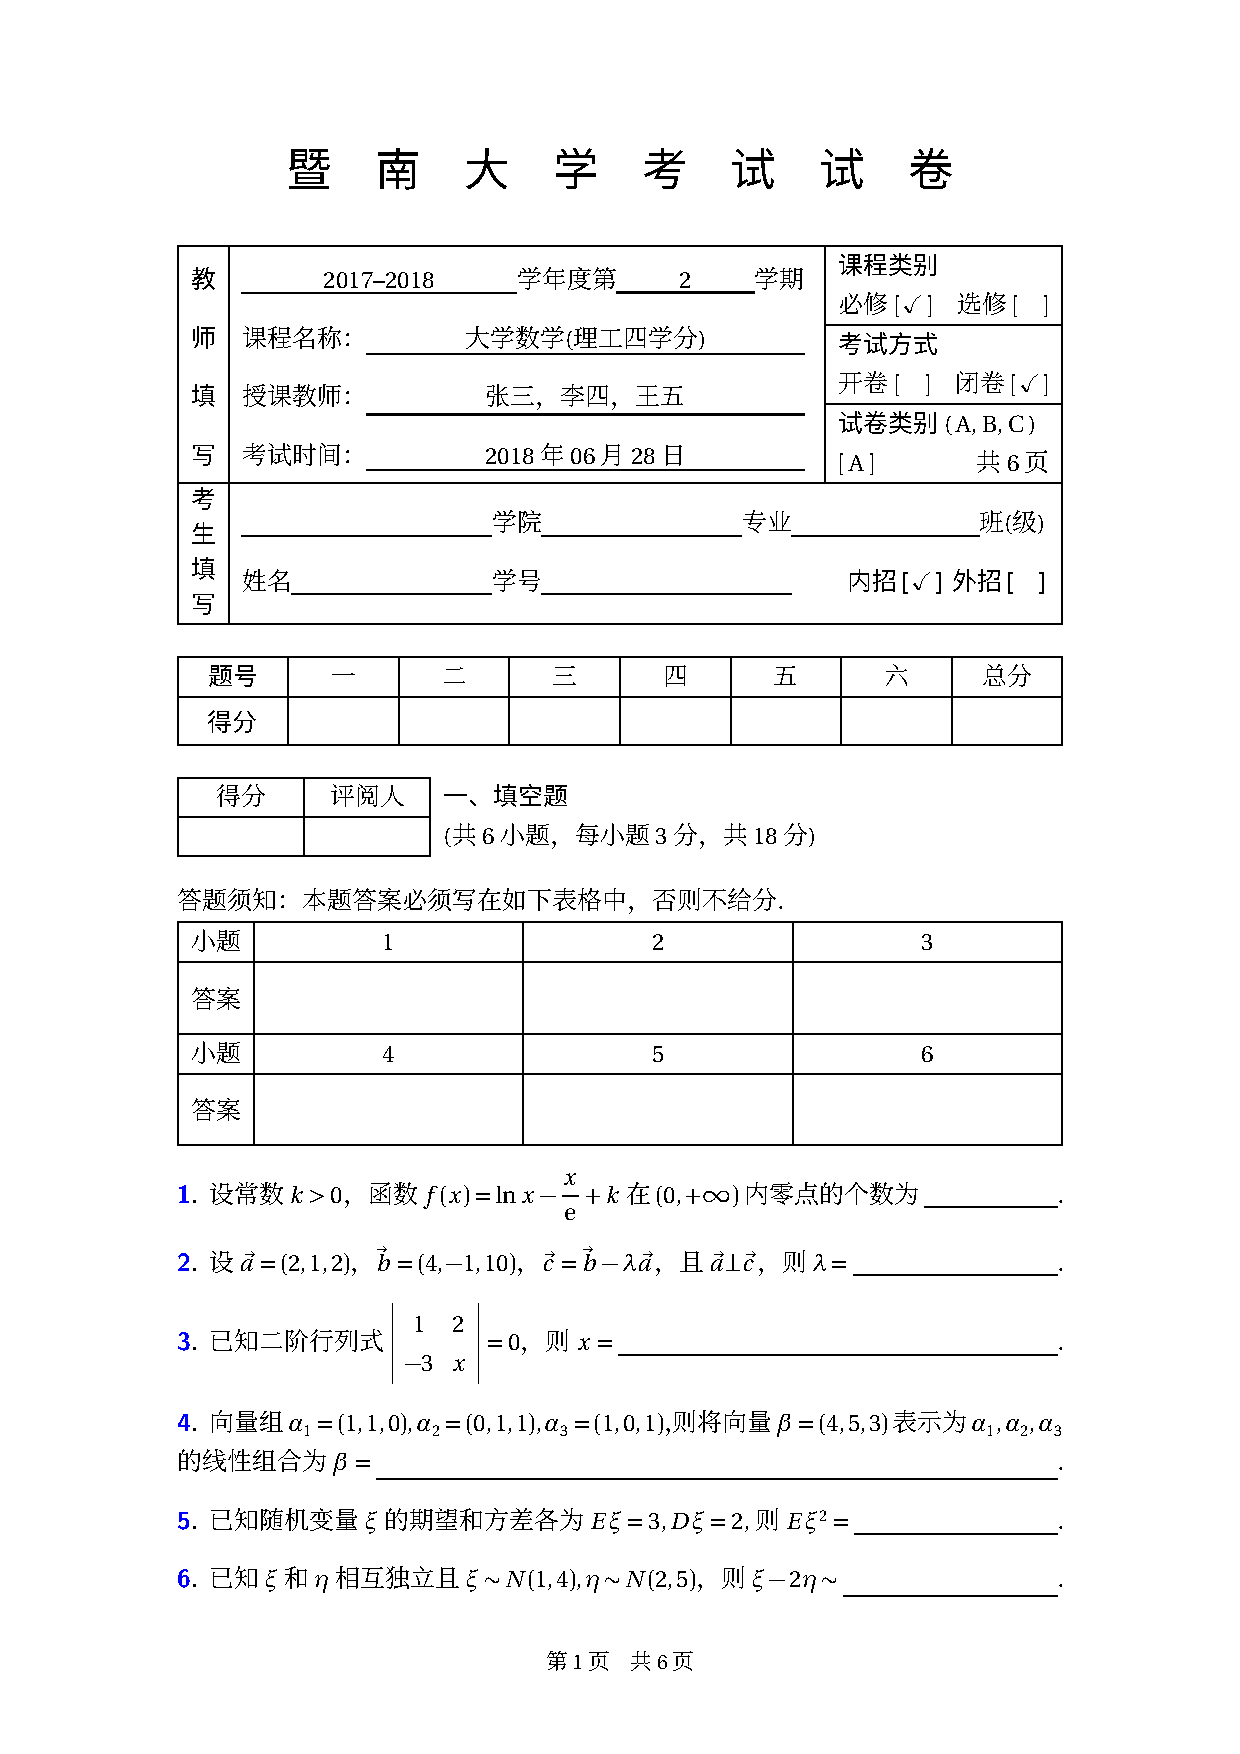
\includepdf[pages=-,nup=2x1]{exam-a-empty}
\end{document}
\end{code}
%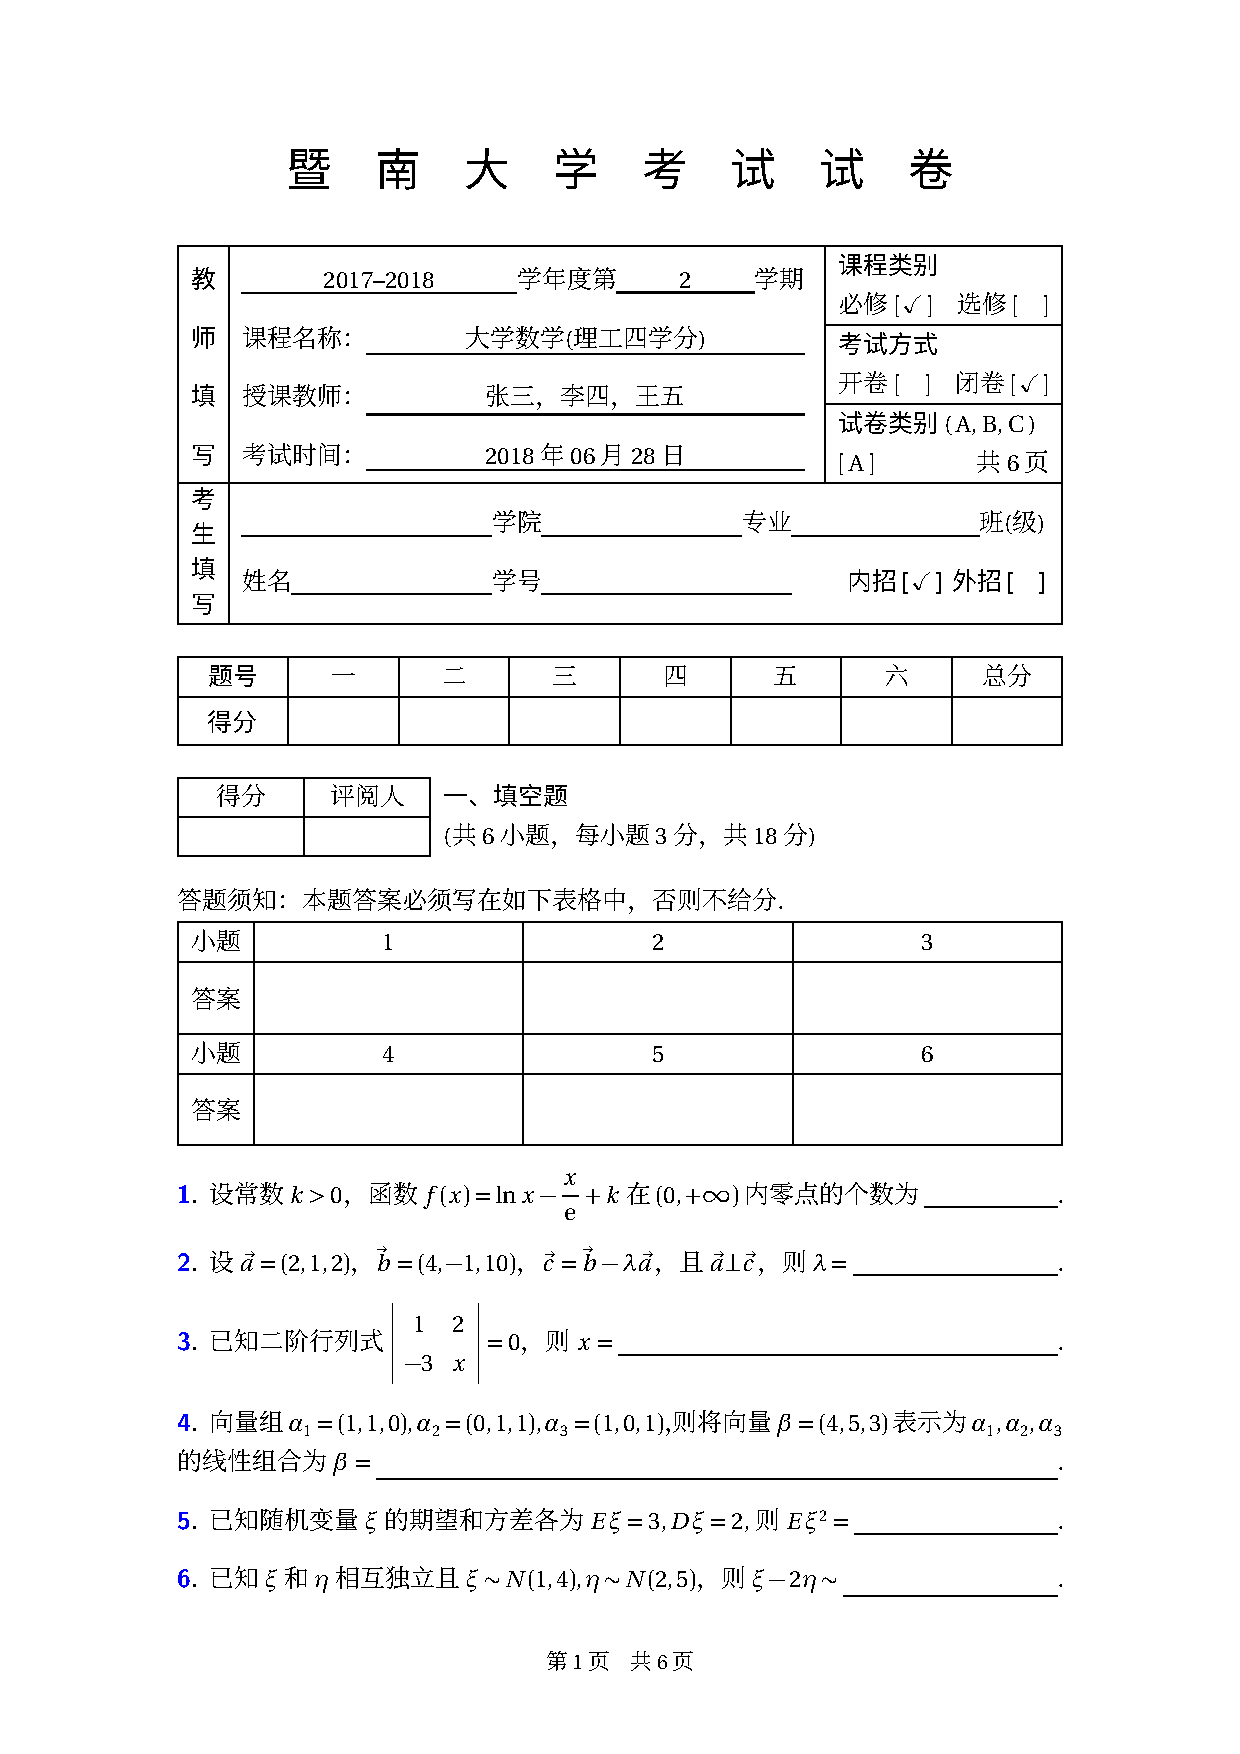
\includepdf[pages=-,nup=2x1,offset=0 0,delta=0 0]{exam-a-empty}
这种用法直接读入 A4 试卷的 PDF 文件,生成双栏的 A3 试卷,适合没有 TeX 文件时使用。
\end{framex}

\end{document}
